\documentclass[tikz,border=2pt]{standalone}
\usepackage{amsmath,amssymb}
\usepackage{tikz}
\usetikzlibrary{arrows.meta}

\begin{document}
% The punctured neighbourhood (x0-δ, x0+δ) \ {x0}: everything within distance δ of x0 except x0
% itself. x0 is a limit point of X when every such neighbourhood still meets X.
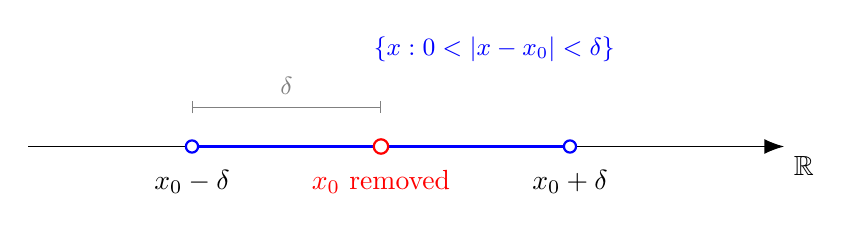
\begin{tikzpicture}[x=1.6cm]
	\draw[-{Latex[length=2.5mm]}] (-2.8,0) -- (3.2,0) node[below right] {$\mathbb{R}$};
	\draw[very thick, blue] (-1.5,0) -- (1.5,0);
	\draw[blue, thick, fill=white] (-1.5,0) circle (2.2pt);
	\draw[blue, thick, fill=white] (1.5,0) circle (2.2pt);
	\draw[red, thick, fill=white] (0,0) circle (2.6pt);
	\node[below=5pt] at (-1.5,0) {$x_0-\delta$};
	\node[below=5pt] at (1.5,0) {$x_0+\delta$};
	\node[red, below=5pt] at (0,0) {$x_0$ removed};
	\draw[gray, |-|] (-1.5,0.5) -- (0,0.5);
	\node[gray, above=1pt, font=\small] at (-0.75,0.5) {$\delta$};
	\node[blue, above=10pt, font=\small] at (0.9,0.6) {$\{x : 0<|x-x_0|<\delta\}$};
\end{tikzpicture}
\end{document}
